\documentclass{article}
% For math environments
\usepackage{amsmath, amsfonts}
% For links
\usepackage[colorlinks=true,
    linkcolor = blue,
    urlcolor  = blue,
    citecolor = blue,
    anchorcolor = blue]{hyperref}
% Put space between paragraphs
\usepackage{parskip}
% For figures
\usepackage{tikz}
% Set the margins to not be ridiculous
\usepackage[margin=0.75in]{geometry}
% For multiple columns
\usepackage{multicol}
% For controlling enum/itemize spacing and indentation
\usepackage{enumitem}
% More math symbols
\usepackage{amssymb}
% To change enumerate labels

% For tikz plots
\usepackage{pgfplots}
% This isn't needed but avoids a compiler warning
\pgfplotsset{compat=1.16}

% Allow multi-line equations to be broken across pages
\allowdisplaybreaks

% Use @ as a letter
\makeatletter

% Scale down all tikz coordinates while maintaining font size
\tikzset{every picture/.style={scale=0.45, every picture/.style={}}}


% Macros
% Monospace code
\def\code#1{\texttt{#1}}

% Greek letters
\def\a{\alpha}
\def\b{\beta}
\def\g{\gamma}
\def\d{\delta}
\def\D{\Delta}

% Commands that make life easier
\newcommand\gath[1]{\begin{gather} #1 \end{gather}}
\newcommand\ali[1]{\begin{align} #1 \end{align}}
\newcommand\parens[1]{\left( #1 \right)}
\newcommand\squares[1]{\left[ #1 \right]}
\newcommand\braces[1]{\left\{ #1 \right\}}
\newcommand\angles[1]{\left\langle #1 \right\rangle}
\newcommand\deriv[2]{\frac{d #1}{d #2}}
\newcommand\abs[1]{\left| #1 \right|}
\newcommand\floor[1]{\left\lfloor #1 \right\rfloor}
\DeclareMathOperator{\lcm}{lcm}
\def\non{\nonumber \\}

% Multiline equation space
\def\mlesp{\hspace{1.2cm}}

% For grid diagrams
\newcommand\gridbox[3]{\draw (#1,#2) rectangle (#1+1,#2+1) node[pos=.5] {#3};}
\newcommand\gridboxh[3]{\draw[fill=red!20] (#1,#2) rectangle (#1+1,#2+1) node[pos=.5] {#3};}
\newcommand\gridboxb[3]{\draw[fill=black] (#1,#2) rectangle (#1+1,#2+1) node[pos=.5] {#3};}
\newcommand\gridsym[3]{\node at (#1+0.5,#2+0.5) {$#3$};}
\newcommand\gridblank[2]{\filldraw[draw=gray, color=gray] (#1,#2) rectangle (#1+1,#2+1);}
\newcommand\gridcirc[2]{\draw (#1 + 0.5,#2 + 0.5) circle (0.25);}
\newcommand\cwlab[3]{
  \def\dd{0.15}
  \draw (#1 + \dd - 0.03, #2 + 1 - \dd) node {\scriptsize #3};
}

\def\bbw{3.5}
\def\bbh{2}
\newcommand\bigbox[3]{\draw (#1*\bbw,#2*\bbh) rectangle (#1*\bbw+\bbw,#2*\bbh+\bbh) node[pos=.5] {#3};}
\newcommand\bbtextr[3]{\node[right] at (#1*\bbw,#2*\bbh+0.5*\bbh) {#3};}
\newcommand\bbtextb[3]{\node[align=center] at (#1*\bbw+0.5*\bbw,#2*\bbh+0.5*\bbh) {#3};}

% Box puzzle stock answer
\newcommand\boxans[1]{
  Logic was used to deduce the solution:

  #1

  This was verified using Python as well as shown to be unique with a brute force approach.
}

% Multiple numbers
\newcommand\mn[1]{$#1$'s}

% Commands for problems
\newcommand\problem[4]{
  \section*{#1}

  Question: #3
  
  Answer: #2
  
  Explanation: #4
}
\newcommand\aproblem[4]{\problem{Dec #1}{#2}{#3}{#4}}
\newcommand\cproblem[4]{\problem{Problem #1}{#2}{#3}{#4}}

\def\advent@xxiv@i{
  Eve writes down five different positive integers.
  The sum of her integers is $16$. What is the product of her integers?
}

\def\advent@xxiv@ii{
  $14$ is the smallest even number that cannot be obtained by rolling two $6$-sided dice and finding the product of the numbers rolled.

  What is the smallest even number that cannot be obtained by rolling one hundred $100$-sided dice and finding the product of the numbers rolled?
}

\def\advent@xxiv@iii{
  There are $5$ ways to write $5$ as the sum of positive odd numbers:
  \begin{itemize}
    \item $1 + 1 + 1 + 1 + 1$
    \item $1 + 1 + 3$
    \item $3 + 1 + 1$
    \item $1 + 3 + 1$
    \item $5$
  \end{itemize}

  How many ways are there to write $14$ as the sum of positive odd numbers?
}

\def\advent@xxiv@iv{
  The geometric mean of a set of $n$ numbers is computed by mulitplying all the numbers together, then taking the $n$th root.
  The factors of $9$ are $1$, $3$, and $9$.
  The geometric mean of these factors is
  \gath{
    \sqrt[3]{1 \times 3 \times 9} = \sqrt[3]{27} = 3
  }
  What is the smallest number where the geometric mean of its factors is $13$?
}

\def\advent@xxiv@v{
  The sum of $11$ consecutive integers is $2024$.
  What is the smallest of the $11$ integers?
}

\def\advent@xxiv@vi{Put the digits 1 to 9 (using each digit exactly once) in the boxes so that the sums are correct. The sums should be read left to right and top to bottom ignoring the usual order of operations. For example, 4+3×2 is 14, not 10. Today's number is the product of the numbers in the red boxes.
  The number $n$ has $55$ digits.
  All of its digits are $9$.
  What is the sum of the digits of $n^3$?
}

\def\advent@xxiv@vii{
  What is the obtuse angle in degrees between the minute and hour hands of a clock at 08:22?
}

\def\advent@xxiv@viii{
  It is possible to arrange $4$ points on a plane and draw non-intersecting lines between them to form $3$ non-overlapping triangles:

  \begin{center}
    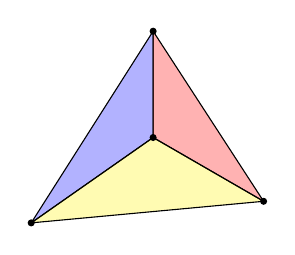
\begin{tikzpicture}
      \def\ds{3}
      \def\pa{(0: 0)}
      \def\pb{(90: \ds)}
      \def\pc{(215: 1.4*\ds)}
      \def\pd{(-30: 1.2*\ds)}

      \def\bcr{3}
      \def\scr{0.55*\bcr}
      \def\sca{34}
      \def\mcr{0.7*\bcr}
      \def\mca{142}
      \def\pr{0.1}

      % Triangles
      \draw[fill=blue,fill opacity=0.3] \pa -- \pb -- \pc -- cycle;
      \draw[fill=red,fill opacity=0.3] \pa -- \pb -- \pd -- cycle;
      \draw[fill=yellow,fill opacity=0.3] \pa -- \pd -- \pc -- cycle;

      % Points
      \fill \pa circle (\pr);
      \fill \pb circle (\pr);
      \fill \pc circle (\pr);
      \fill \pd circle (\pr);
    \end{tikzpicture}
  \end{center}

  It is not possible to make more than $3$ triangles with $4$ points.

  What is the maximum number of non-overlapping triangles that can be made by arranging $290$ points on a plane and drawing non-intersecting lines between them?
}

\def\advent@xxiv@ix{
  Put the digits $1$ to $9$ (using each digit exactly once) in the boxes so that the sums are correct.
  The sums should be read left to right and top to bottom ignoring the usual order of operations.
  For example, $4 + 3 \times 2$ is $14$, not $10$.
  Today's number is the product of the numbers in the red boxes.

  \grid@advent@xxiv@ix{}{}{}{}{}{}{}{}{}
}

\def\advent@xxiv@x{
  A number is a palindrome if it's the same when its digits are written in reverse order.

  What is the sum of all the numbers between $10$ and $100$ that are palindromes?
}

\def\advent@xxiv@xi{
  There are $6$ sets of integers between $1$ and $5$ (inclusive) that contain an odd number of numbers whose median value is $3$:

  \begin{itemize}
    \item $\braces{3}$
    \item $\braces{1,3,4}$
    \item $\braces{2,3,4}$
    \item $\braces{1,3,5}$
    \item $\braces{2,3,5}$
    \item $\braces{1,2,3,4,5}$
  \end{itemize}

  How many sets of integers between $1$ and $11$ (inclusive) are there that contain an odd number of numbers whose median value is $5$?
}

\def\advent@xxiv@xii{
  Holly picks a three-digit number.
  She then makes a two-digit number by removing one of the digits.
  The sum of her two numbers is $309$.
  What was Holly's original three-digit number?
}

\def\advent@xxiv@xiii{
  Today's number is given in this crossnumber.
  No number in the completed grid starts with $0$.

  \begin{multicols}{2}
    \crossnumstd{}{}{}{}{}{}{}{}{}

    \vfill\null
    \columnbreak

    \begin{center}
      \textbf{Across}

      \begin{tabular}{clc}
        \textbf{1} & Today's number.  & (\textbf{3}) \\
        \textbf{4} & Two times 5A.    & (\textbf{3}) \\
        \textbf{5} & A multiple of 1. & (\textbf{3})
      \end{tabular}

      \textbf{Down}

      \begin{tabular}{clc}
        \textbf{1} & Sum of digits is 15. & (\textbf{3}) \\
        \textbf{2} & Sum of digits is 19. & (\textbf{3}) \\
        \textbf{3} & Three times 5A.      & (\textbf{3})
      \end{tabular}
    \end{center}
  \end{multicols}
}

\def\advent@xxiv@xiv{
  $15^3$ is $3375$.
  The last $3$ digits of $15^3$ are $375$.

  What are the last $3$ digits of $15^{1234567890}$?
}

\def\advent@xxiv@xv{
  The number $2268$ is equal to the product of a square number (whose last digit is not $0$) and the same square number with its digits reversed: $36 \times 63$.

  What is the smallest three-digit number that is equal to the product of a square number (whose last digit is not $0$) and the same square number with its digits reversed?
}

\def\advent@xxiv@xvi{
  Put the digits $1$ to $9$ (using each digit exactly once) in the boxes so that the sums are correct.
  The sums should be read left to right and top to bottom ignoring the usual order of operations.
  For example, $4 + 3 \times 2$ is $14$, not $10$.
  Today's number is the product of the numbers in the red boxes.

  \grid@advent@xxiv@xvi{}{}{}{}{}{}{}{}{}
}

\def\advent@xxiv@xvii{
  The number $40$ has $8$ factors: $1$, $2$, $4$, $5$, $8$, $10$, $20$, and $40$.

  How many factors does the number $2^{26} \times 5 \times 7^5 \times 11^2$ have?
}

\def\advent@xxiv@xviii{
  TODO
}

\def\card@xxiv@i{
  What is the largest number you can make by using the digits $1$ to $4$ to make two $2$-digit numbers, then mutiplying the two numbers together?
}

\def\card@xxiv@ii{
  What is the largest number you can make by using the digits $0$ to $9$ to make a $2$-digit number and an $8$-digit number, then mutiplying the two numbers together?
}

\def\card@xxiv@iii{
  The expansion of $(2x+3)^2$ is $4x^2 + 12x + 9$.
  The sum of the coefficients of $4x^2 + 12x + 9$ is $25$.
  What is the sum of the coefficients of the expansion of $(30x + 5)^2$?
}

\def\card@xxiv@iv{
  What is the sum of the coefficients of the expansion of $(2x+1)^{11}$?
}

\def\card@xxiv@v{
  What is the geometric mean of all the factors of $41306329$?
}

\def\card@xxiv@vi{
  What is the largest number for which the geometric mean of all its factors is $92$?
}

\def\card@xxiv@vii{
  What is the sum of all the factors of $7^4$?
}

\def\card@xxiv@viii{
  How many numbers between $1$ and $28988500000$ have an odd number of factors?
}

\def\card@xxiv@ix{
  Eve found the total of the $365$ consecutive integers starting at $500$ and the total of the next $365$ consecutive integers, then subtracted the smaller total from the larger total.
  What was her result?
}

\def\card@xxiv@x{
  Eve found the total of the $n$ consecutive integers starting at a number and the total of the next $n$ consecutive integers, then subtracted the smaller total from the larger total.
  Her result was $22344529$.
  What is the largest possible value of $n$ that she could have used?
}


\begin{document}

\title{Matthew Scroggs 2020 Christmas Card Solutions}
\author{Dan Whitman}
\date{}

\maketitle

Link to the online card: \href{https://www.mscroggs.co.uk/blog/87}{https://www.mscroggs.co.uk/blog/87}

\cproblem{1}{1304}{\card@xx@i}{
  The number of $r$-digit numbers formed using these digits is the number of permutations of the 6 digits, selecting $r$ of them.
  If interested only in the odd numbers, the least significant digit must only be chosen from the 4 odd digits (1, 3, 5, and 7) whereas the rest are chosen normally from the remaining digits.
  Thus the total number of odd numbers is reasoned to be
  \gath{
    \sum_{r=1}^5 \frac{4 \cdot 5!}{6 - r} = 1304 \,.
  }

  This answer was also verified using a brute force Python program.
}

\cproblem{2}{322402}{\card@xx@ii}{
Each sheet of paper has four numbers on it.
For example, the bottom sheet would have the numbers 1 and 2 on the front half and 161199 and 161200 on the back half.
In general, it is reasoned the that $n$th sheet, where the bottom is sheet 1, has the following numbers on it:
\ali{
  & 2n -1 &
  & 2n &
  & N - 2(n-1) - 1 &
  & N - 2(n-1) \,,
}
where $N = 161200$.
Therefore the sum of the numbers on the $n$th sheet is
\ali{
s_n &= [2n - 1] + [2n] + [N - 2(n-1) - 1] + [N - 2(n-1)] \non
&= 4n - 2 + 2N - 4(n-1) \non
&= 4n - 2 + 2N - 4n + 4 \non
&= 2N + 2 \non
&= 2(N+1) \non
&= 322402 \,.
}
So evidently all sheets have this same sum, which means that it is of course also the largest number since it is the only number!

This answer was also verified using a brute force Python program.
}

\cproblem{3}{4249475344}{\card@xx@iii}{
  Let $N = 65188$ so that $2N - 1 = 130375$ is clearly the largest odd number between these.
  The sum of all odd numbers between is then reasoned to be
  \ali{
    s &= \sum_{n=1}^N (2n - 1) = \sum_{n=1}^N 2n - \sum_{n=1}^N 1 = 2 \sum_{n=1}^N n - N \non
    &= 2 \frac{N(N+1)}{2} - N = N(N+1) - N = N^2 + N - N \non
    &= N^2 = 4249475344
  }

  This answer was also verified using a brute force Python program.
}

\cproblem{4}{51}{\card@xx@iv}{
  Suppose that the values on the the cards are $a$, $b$, and $c$.
  Then we have the following equations
  \ali{
    a + b &= 31 &
    a + c &= 35 &
    b + c &= 46 \,,
  }
  noting that it does not matter which of the variables corresponds to which card since there are only three.
  We then have that
  \gath{
    (a + b) + (a + c) + (b + c) = 31 + 35 + 46 = 102 \non
    2a + 2b + 2c = 102 \non
    2(a + b + c) = 102 \non
    a + b + c = 51
  }
  We could also solve the above system of linear equations directly using matrices:
  \gath{
    \begin{bmatrix}
      1 & 1 & 0 \\
      1 & 0 & 1 \\
      0 & 1 & 1
    \end{bmatrix}
    \begin{bmatrix}
      a \\ b \\ c
    \end{bmatrix}
    =
    \begin{bmatrix}
      31 \\ 35 \\ 36
    \end{bmatrix} \,.
  }
  This results in the numbers on the cards being $a = 15$, $b = 16$, and $c = 20$ so that again their sum is the same as before.
}

\cproblem{5}{4011}{\card@xx@v}{
  Suppose that the square base of the pyramid has sides $s$ and the pyramid has a height $h$.
  Then the formula for its volume, which we are given, is
  \gath{
    V_p = \frac{h s^2}{3} = 1337 \,.
  }
  Clearly the smallest cuboid containing the pyramid has dimensions of $s \times s \times h$ so that its volume is
  \gath{
    V_c = h s^2 \,.
  }
  Therefore
  \gath{
    \frac{V_c}{3} = \frac{h s^2}{3} = V_p \non
    V_c = 3 V_p = 4011 \,.
  }
}

\cproblem{6}{3355}{\card@xx@vi}{
  Letting $a = 305$ and $b = 671$, we have that $\gcd(a,b) = 61$.
  Hence the lowest common multiple is
  \gath{
    \lcm(a,b) = \frac{ab}{\gcd(a,b)} = 3355 \,.
  }
}

\cproblem{7}{2305}{\card@xx@vii}{
  For $n$ dice, the minimum possible sum is $n$ when they all roll a one.
  The maximum number is $6n$ when they all roll a six.
  Every sum $s$ such that $n \leq s \leq 6n$ is possible and occurs some number of times in the $6^n$ possible dice combinations.
  Obviously the sums $s = n$ and $s = 6n$ each occur only once.
  Let $N_n(s)$ be the number of combinations that sum $s$ occurs in the rolls of $n$ dice, which is of course directly related to the probability of that sum occurring.
  Though I was unable to prove it, some numerical experiments showed that all the values of $s$ are symmetric such that
  \gath{
    N_n(n + i) = N_n(6n - i)
  }
  for all integer $0 \leq i \leq 5n$.

  Letting $a = 6136$ and $b = 9999$, there must then be some integers $n$ and $i$ such that
  \ali{
    n + i &= a \\
    6n -i &= b
  }
  since these sums have the same probability.
  Thus this linear system can be solved:
  \gath{
    \begin{bmatrix}
      1 & 1  \\
      6 & -1
    \end{bmatrix}
    \begin{bmatrix}
      n \\ i
    \end{bmatrix}
    =
    \begin{bmatrix}
      a \\ b
    \end{bmatrix} \,.
  }
  Doing so results in $n = 2305$ and $i = 3830$, where of course $n$ is the number of dice and so is our answer.
}

\cproblem{8}{1225}{\card@xx@viii}{
For an $n \times m$ grid, it is reasoned that the number of different squares with sides of $k$ spaces is
\gath{
  N_k = (n - k + 1)(m - k + 1) \,,
}
assuming that $n \geq k$ and $m \geq k$ (where $N_k = 0$ otherwise since no $N_k$ squares can fit in the grid).
Letting $p = \min(n,m)$, it is reasoned that the total number of squares in the grid is
\ali{
N &= \sum_{k=1}^{p} N_k = \sum_{k=1}^p (n - k + 1)(m - k + 1) = \sum_{k=1}^p [n - (k - 1)][m - (k - 1)] \non
&= \sum_{k=0}^{p-1} (n - k)(m - k) = \sum_{k=0}^{p-1} \left[nm - k(n + m) + k^2\right] \non
&= nm \sum_{k=0}^{p-1} 1 - (n + m) \sum_{k=0}^{p-1} k + \sum_{k=0}^{p-1} k^2 \non
&= pnm - (n + m) \frac{p(p-1)}{2} + \frac{p(p-1)(2p-1)}{6} \non
&= pnm + \frac{p(p-1)}{6} \left(2p - 3n - 3m - 1\right)
}
noting that this formula is symmetric with respect to $n$ and $m$, which is to be expected.
In our case of course $n = 14$ and $m = 16$ so that $p = \min(14, 16) = 14$, which results in $N = 1225$.

The sum was also verified in its original form with Python.
}

\cproblem{9}{141516}{\card@xx@ix}{
  First, since the sum is odd, it has to be that the least significant digit was the one that was removed, since otherwise the last digit of the sum would be even.
  So, if $x$ is the original number and $d_0$ is its last digit, then the second number is
  \gath{
    y = \frac{x - d_0}{10} \,.
  }
  Hence the sum of these numbers is
  \gath{
    s = x + y = x + \frac{x - d_0}{10} = 155667 \non
    10x + x - d_0 = 10s \non
    11x = 10s + d_0 \,.
  }
  Hence we merely need to find the digit $d_0$ such that $10s + d_0$ is divisible by $11$, of which there are 10 possibilities since $d_0 \in \{0,1,\ldots,8,9\}$.
  This was checked using a Python program, which found that this condition is met only when $d_0 = 6$ so that the original number must be $x = (10s + d_0)/11 = 141516$.
}

\end{document}
